The projective plane is an idea that grew out of the renaissance study of perspective in art.
For example, when stood between two railway lines, they appear to meet at the horizon. \Cref{projective-parallel} is a rudimentary diagram of the situation.
While this is merely a trick of perspective in euclidean space, in the projective plane, parallel lines \emph{do} meet, at a so called `point at infinity'.
The idea is to add these points at infinity to the euclidean plane so that each line contains exactly one.
On top of this is the one exception, the `line at infinity', which is defined to be the unique line that is simply the collection of all points at infinity.
These ideas, while formative, are hardly rigorous, and we present the proper definition and constructions (there are two) of projective space below.

\begin{figure}[htpb]
	\centering
	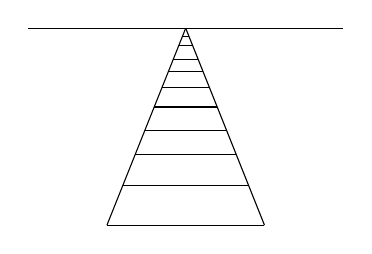
\begin{tikzpicture}[scale=0.5]
		% railway lines
		\draw (-2,0) -- (0,5);
		\draw (2,0) -- (0,5);
		% sleepers. To work out an appropriate x for given y, x=2(1-(y/5))
		\draw (-2,0) -- (2,0);
		\draw (-1.6,1) -- (1.6,1);
		\draw (-1.28,1.8) -- (1.28,1.8);
		\draw (-1.04,2.4) -- (1.04,2.4);
		\draw (-0.8,3) -- (0.8,3);
		\draw (-0.6,3.5) -- (0.6,3.5);
		\draw (-0.44,3.9) -- (0.44,3.9);
		\draw (-0.32,4.2) -- (0.32,4.2);
		\draw (-0.18,4.55) -- (0.18,4.55);
		\draw (-0.08,4.8) -- (0.08,4.8);
		% horizon
		\draw (-4,5) -- (4,5);
	\end{tikzpicture}
	\caption{Parallel lines `meeting' at infinity in euclidean space}
	\label{projective-parallel}
\end{figure}

\begin{definition}
	The projective plane is an extension of regular 2-dimensional euclidean space by adding `points at infinity' such that every pair of lines intersects exactly once. Points in the projective plane are represented as triples of homogeneous coordinates [X,Y,Z]. More generally, points in projective $n$-space are represented by $n+1$-tuples, such that not all coordinates are zero.
\end{definition}

The two constructions of projective space give two different interpretations of it, both of which are useful to consider.
% perhaps explain affine space (haha) too?
Projective $n$-space can be thought of as either affine $n$-space with points at infinity added (mentioned already) or as a quotient of affine $(n+1)$-space.

\subsubsection{Construction 1: Quotient of $\an[n+1]$}
Remove the origin (i.e. the point $(0,0,\ldots,0)$) from $\an[n+1]$ and define an equivalence relation $\sim$ on the remaining points as follows:
$$(a_0,a_1,\ldots,a_n) \sim (b_0,b_1,\ldots,b_n) \iff (a_0,a_1,\ldots,a_n) = \lambda(b_0,b_1,\ldots,b_n) = (\lambda b_0,\lambda b_1,\ldots,\lambda b_n)$$
where $\lambda$ is a non-zero scalar. Then we have 
$$\pn = (\an[n+1]\setminus\{(0,\ldots,0)\})/\sim,$$
the set of equivalence classes of $\sim$.

For points in $\pn$, write $P = [p_0,p_1,\ldots,p_n]$, where the square brackets represent \emph{homogeneous coordinates}.
By the nature of this construction, we see that scaling homogeneous coordinates results in coordinates of the same point.
Therefore, for a given point, there is no unique representation in homogeneous coordinates.

\subsubsection{Construction 2: Extension of $\an[n]$}
Now we present the second construction of $\pn$, which can be thought of as adding points at infinity to euclidean space.
This is done inductively on $n$ by defining maps $\alpha_n$ and $\beta_n$.
To begin with, let $\pn[0] = \an[1] \setminus \{0\}$ and let
\begin{alignat*}{2}
&\alpha_n : \an \rightarrow \pn,\quad &&\alpha_n(x_1,\ldots,x_n) = [x_1,\ldots,x_n,1]\\
 &\beta_n : \pn[n-1] \rightarrow \pn,\quad &&\beta_n[X_1,\ldots,X_n] = [X_1,\ldots,X_n,0]
\end{alignat*}
Then we can define
$$\pn = \alpha_n(\an) \cup \beta_n(\pn[n-1])$$
Effectively, we have that $\alpha_n$ is the embedding of affine space in $\pn$ and $\beta_n$ represents the points at infinity of $\pn$.
Notice that the image of $\beta_n$ will always give valid homogeneous coordinates, as we removed zero from $\pn[0]$, and therefore at least one of the first $n$ coordinates will be nonzero.
\subsubsection{Homogenisation of Functions}
Since homogeneous coordinates are not unique, it is not always possible to define curves in projective space in the usual form of $F(X,Y,Z)=0$. To that extent, when working with the projective plane, it is convenient to define a homogeneous function as a function which satisfies
$$F(tX_1,tX_2,\ldots,tX_n)=t^k F(X_1,X_2,\ldots,X_n)$$
for some $k$. We see that these kinds of functions \emph{are} well-defined in the projective plane, since
$$F(X_1,X_2,\ldots,X_n)=0 \Leftrightarrow F(tX_1,tX_2,\ldots,tX_n) = t^k F(tX_1,tX_2,\ldots,tX_n) = 0$$
For this document, we need only focus on polynomials, and it is easy enough to see that a polynomial is homogeneous if and only if the degree of each monomial $= d$, for some $d \in \N$.
So the polynomial $\frac{1}{2}x^4 + x^2y^2 + 14xy^3$ is homogeneous with degree 4, whereas the polynomial $17x^5 + 12x^2y + 2$ is not, as the monomials have degrees 5, 3 and 0, from left-to-right.

It is possible to homogenise a given polynomial $F(x_1,\ldots,x_n)$ by letting $F' = F'(x_0,x_1,\ldots,x_n) = x_0^d F(\frac{x_1}{x_0},\ldots,\frac{x_n}{x_0})$, where $d$ is the maximum degree of all monomials of $F$. In practice, this resembles `topping up' the monomials with an extra variable as necessary.
So the inhomogeneous polynomial $17x^5 + 12x^2y + 2$ discussed earlier can be homogenised as $17X^5 + 12X^2YZ^2 + 2Z^5$. There are a few things to notice here. First, when writing out projective polynomials, we use uppercase letters to distinguish them from affine variables and make the context clear. We also use $x$, $y$ and $z$ (and also $X$, $Y$ and $Z$) as the three variables when dealing with the projective plane (uppercase) and the affine part thereof (lowercase).

To summarise, it is possible to move to and from the projective plane with regards to both points and polynomials. A point $(x,y)$ can be mapped to $[x,y,1]$, and a polynomial such as $x^2 + y$ can be mapped to $X^2 + YZ$.

\begin{figure}[htpb]
	\centering
	\begin{tikzpicture}[scale=0.5,domain=-5:5]
		% axes
		\draw[->] (-5,0) -- (5,0);
		\draw[->] (0,-5) -- (0,5);
		% lines
		\draw 
		plot (\x, {0.5*\x+1});
		\draw 
		plot (\x, {0.5*\x+4});
		% annotation
		\draw[dashed,->]
		plot (\x, {0.5*\x+2.5});
		\node [right] at (5,5) {[3,-2,0]};
	\end{tikzpicture}
	\caption{The intersection of $2x - 3y + 1 = 0$ and $2x - 3y + 4 = 0$}
	\label{euclidean-intersection}
\end{figure}
The lines given by $2x - 3y + 1 = 0$ and $2x - 3y + 4 = 0$, which are parallel in $\R^2$, intersect in the projective plane at the point [3,-2,0].
This is because, when homogenised with respect to $z$, the curves are given by $2X - 3Y + Z = 0$ and $2X - 3Y + 4Z = 0$, which are clearly satisfied by $[X,Y,Z] = [3,-2,0]$.
